\chapter{UV-VIS spectra}

The synthesized complexes were investigated via UV-VIS-sprectroscopy. No absorption bands were observed in the UV-Vis-spectra of the colorless complexes of Zn and Cd. Cobalt and azide-copper complexes showed three and one absorption band, respectively. The spectra are shown in  the appendix  and the absorption bands of cobalt complexes are found in table \ref{tab:absorp}.\\


\begin{table}[htpb!]
\centering
\captionabove{Absorption bands of  cobalt complexes in nm}
\begin{tabular}{|l|l|l|l|l|}
\hline
complex & structure & v$_3$ & v$_2$ & v$_1$\\
\hline
Co(N$_3$)$_2$(4-Me-O-py)$_4$ & octahedral & 337 & 505 & 1137\\
\hline
Co(OCN)$_2$(4-Me-O-py)$_4$ & octahedral & 302 & 484 & 1063\\
\hline
Co(SCN)$_2$(4-Me-O-py)$_4$ & octahedral & 324 & 494 & 1049\\
\hline
Co(dca)$_2$(4-HO-Me-py)$_2$ & octahedral &  314 & 483 & 1051\\
\hline
\end{tabular}
\label{tab:absorp}
\end{table}











 The ligand-field  splitting parameter Dq and the Racah-parameter B \cite{racah} were calculated for  Co complexes (d$^7$ with octahedral structure) using eq. \ref{eq:Dq} and \ref{eq:B}.


\begin{equation}
34 Dq^2 + 18 (v_2-2*v_1) Dq + v_{1}^{2}-v_1 * v_2 = 0
\label{eq:Dq}
\end{equation}

\begin{equation}
B = \frac{v_2 - 2 v_1 +30 Dq}{15}
\label{eq:B}
\end{equation}

The calculated Dq and B-values are listed  in table \ref{tab:Racah}.
The allowed transitions are \ce{^4T_{1g}(F) \rightarrow ^4T_{2g}(F)}, \ce{^4T_{1g}(F) \rightarrow ^4T_{2g}(P)}  and \ce{^4T_{1g}(F) \rightarrow ^4A_{2g}}. The Co complexes don't possess perfect octahedral structures, therefore the calculated Dq and B-values don't fit in the Tanabe-Sugano-diagramm in figure \ref{fig:TSD}

\begin{table}[htpb!]
\centering
\captionabove{Dq and Racah-parameter(B) of the Co complexes in cm$^{-1}$}
\begin{tabular}{|l|l|l|l|l|}
\hline
complex &Dq & B\\
\hline
Co(N$_3$)$_2$(4-Me-O-py)$_4$ & 478 & 1104\\
\hline
Co(OCN)$_2$(4-Me-O-py)$_4$ &  511 & 1146\\
\hline
Co(SCN)$_2$(4-Me-O-py)$_4$ & 518 & 1113 \\
\hline
Co(dca)$_2$(4-HO-Me-py)$_2$ & 517  & 1145\\
\hline
\end{tabular}
\label{tab:Racah}
\end{table} 



 
\begin{figure}
\centering
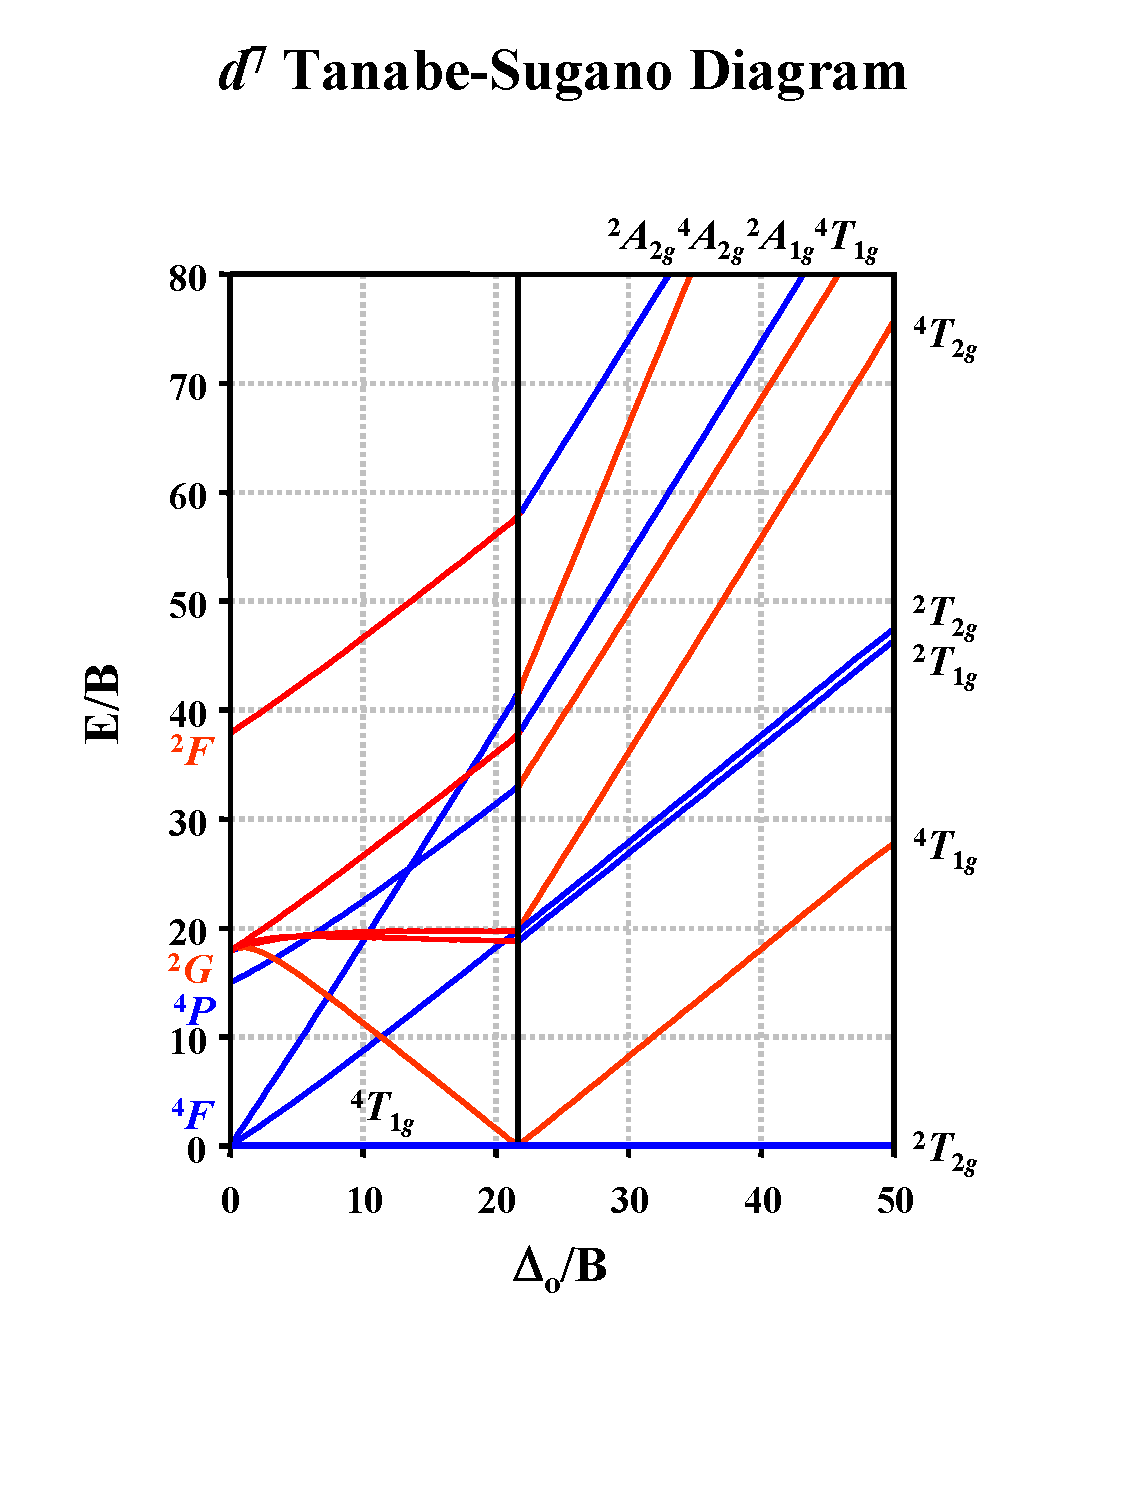
\includegraphics[trim= 14mm 34mm 24mm 35mm, clip, width=0.8\textwidth]{figures/TSdiagram_06.pdf}
\caption[Tanabe-Sugano-Diagramm]{Tanabe-Sugano-Diagramm of the d$^7$- configuration of an octahedral structure \cite{tansug}}
\label{fig:TSD}
\end{figure}




